\documentclass[11pt]{article}

\usepackage[a4paper,left=3cm,right=3cm,top=2cm,bottom=2cm,bindingoffset=5mm]{geometry}
\usepackage{ngerman}
\usepackage[ngerman]{babel}
\usepackage[ansinew]{inputenc}
\usepackage[T1]{fontenc}
\usepackage[scaled]{uarial}
\usepackage{fancyhdr}
\usepackage{wrapfig}
%Baumstrukturen
\usepackage{tikz}
\usepackage{tikz-qtree}
\usepackage{textcomp}   % allows \textrightarrow
%Mathe
\usepackage{amsmath}

%Item mit Pfeil
\newcommand{\aitem}{%
\item[$\rightarrow$]
}

\title{Die augusteische Baupolitik}
\author{Florian Seligmann}
\date{Montag, 11. Juni 2018}

\pagestyle{fancy}
\lhead{GFS von Florian Seligmann}
\rhead{11. Juni 2018}
\chead{}

%----------------------------------------------------------------------------------------------------------
\begin{document}

\begin{center}
%\vspace*{\stretch{1.0}}
   \begin{center}
      \Large\textbf{Die augusteische Baupolitik}\\
      \large\textit{Florian Seligmann}
   \end{center}
%\vspace*{\stretch{2.0}}

\small

\section{Zeit der B�rgerkriege}
\begin{itemize}
	\item Betonung Roms im Gegensatz zu Marcus Antonius (z.B. Augustusmausoleum)
	\item Caesarkult (z.B. Curia Iulia, Tempel des Divus Iulius)
	\item Bezug zu Apollo
	\aitem Repr�sentative Bauten in Rom
\end{itemize}

\section{Zeit des Prinzipats}
\begin{itemize}
	\item Fertigstellung und Sanierung vieler Bauwerke und der Infrastruktur (Brandschutz, Wasserversorgung, \dots)
	\item Bau und Erneuerung vieler Tempel
	\aitem Dabei Verwendung von teurem Marmor zur Repr�sentation des weltweiten Einfluss
	\aitem Betonung der \glqq{}aetas aurea\grqq{}
	\aitem Dadurch ausgel�ster \glqq{}Wettbewerb\grqq{} unter der Elite $\rightarrow$ Goldenes Zeitalter wird sichtbar
	\aitem Ziel: Darstellung als Friedensbringer (Schlie�ung des Tempel des Ianus Quirinum, Bau der Ara Pacis, \dots)
\end{itemize}

\section{Ara Pacis Augustae}

\vspace*
\begin{itemize}
	\item Errichtet vom Senat wegen Augustus R�ckkehr von Feldz�gen in Spanien und Gallien
	\item Errichtet auf dem Marsfeld neben Augustusmausoleum und Ara Pacis
	\item Geweiht am Geburtstag seiner Frau Livia
	\item Aufbau �hnlich einem templum minus $\rightarrow$ Aber aus massivem lunensichem Marmor (= Carrara-Marmor)
	\item Heute als Rekonstruktion im Museo dell'Ara Pacis
\end{itemize}

\begin{wrapfigure}{r}{0.3\textwidth}
	\begin{center}
		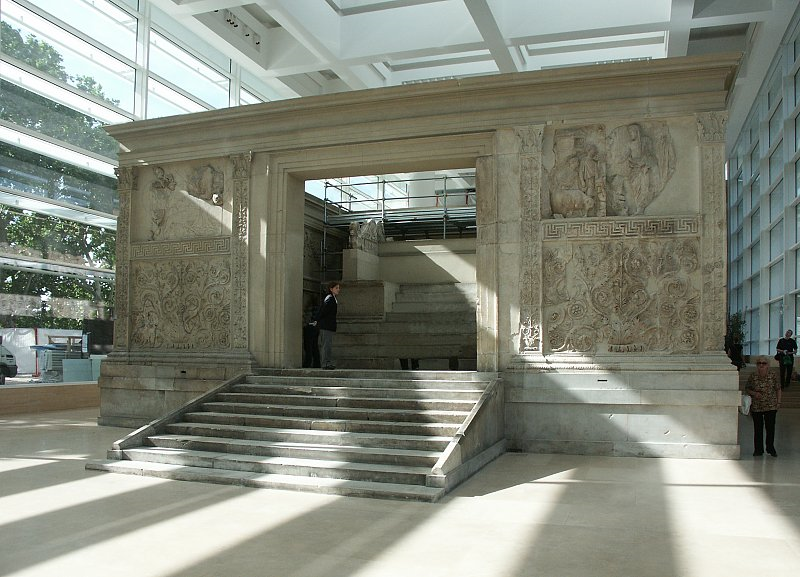
\includegraphics[width=0.48\textwidth]{images/ap_totale.png}
		
	\end{center}
\end{wrapfigure}

\subsection{Aufgaben}
\begin{itemize}
	\item R�ckblick auf Griechenland \& die Republik
	\item Ausblick auf \glqq{}Goldenes Zeitalter\grqq{}
\end{itemize}

\subsection{Gestaltung}
\begin{itemize}
	\item 
\end{itemize}

\end{center}
\end{document}